\section{Investigation of a Single Inverter Module}
\label{chap:curr_driven_rect}

\subsection{Effect on Power Device Stress}

As shown in Fig. \ref{fig:SingleModuleInductanceMap}, the power loop includes two switches and the phase capacitor. When the phase current transfers from one switch to the other, the power loop parasitic inductances cause either a voltage overshoot on the drain-source terminals of a switch as much as $L_p*di/dt$. Considering the high current rise and fall time capability of GaN FETs, i.e. high di/dt, the power loop inductance is the most important factor for device stress. Experimental results of device stress can be seen in Fig. \ref{fig:experimentalvds2} for different DC link voltages. It has been shown that the peak stress on phase-B is higher since its power loop equivalent inductance is slightly larger than phase-A.

\subsection{Effect on DC link Capacitor Stress}

The DC link capacitors placed on each half-bridge are used to supply and sink the current ripple during switching periods. The power loop inductances are not effective on these capacitors' stress assuming ceramic capacitors are placed in much closer proximity.
When the parasitic inductances are of considerable amount on the commutation loop, the stress of individual capacitors increase due to the longer path which the other capacitors have, as shown in Fig. \ref{fig:single_module_curr_ripple}. This results in higher capacitor RMS currents than analytically calculated \cite{Ugur2017} as shown in Fig. \ref{fig:CapacitorCurrentRMS} and must be taken into account as the selected capacitor temperature may increase too much, eventually shortening its lifetime. On the other hand, this effect is not significantly reflected to the voltage ripple.

\begin{figure}[tb]
\minipage{0.49\textwidth}
  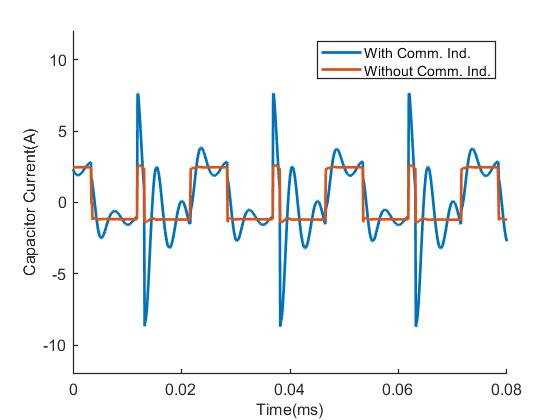
\includegraphics[width=\linewidth]{figures/single_module_curr_ripple.jpg}
  \caption{DC bus capacitor current ripple with and without commutation loop inductances}\label{fig:single_module_curr_ripple}
\endminipage\hfill
\minipage{0.49\textwidth}
  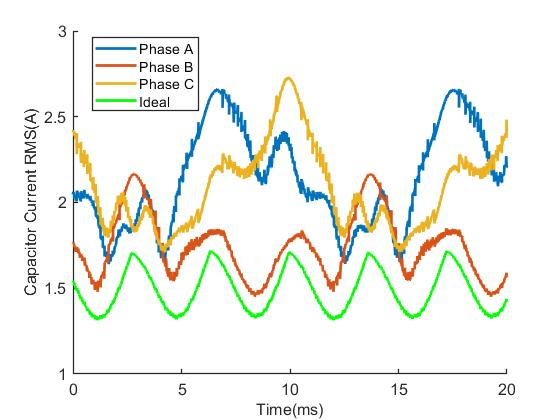
\includegraphics[width=\linewidth]{figures/CapacitorCurrentRMS.jpg}
  \caption{Variation of RMS values of capacitor currents with and without commutation inductances}\label{fig:CapacitorCurrentRMS}
\endminipage
\end{figure}


